\documentclass{article}
\usepackage[utf8]{inputenc}
\usepackage[spanish]{babel}
\usepackage{graphicx}
\usepackage{float}
\usepackage{pdfpages}
\graphicspath{{./img/}}

\title{Práctica 2. Segunda parte. Ingeniería de requisitos: Modelo de casos de uso}
\author{Eugenio Alcántara García\\
		\and Noelia Escalera Mejías\\
		\and Alejandro Menor Molinero\\
		\and Jesús Torres Sánchez}
	
\begin{document}
	\maketitle
	\section{Plantillas de Casos de Uso extendidas}
	\begin{figure}[H]
		\centering
		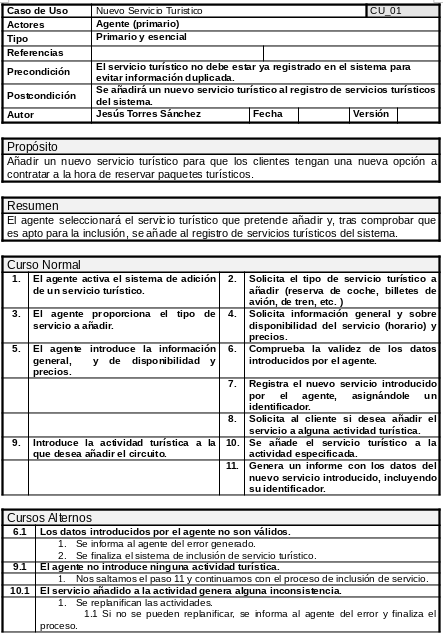
\includegraphics[totalheight=12cm]{cu-1}
	\end{figure}
	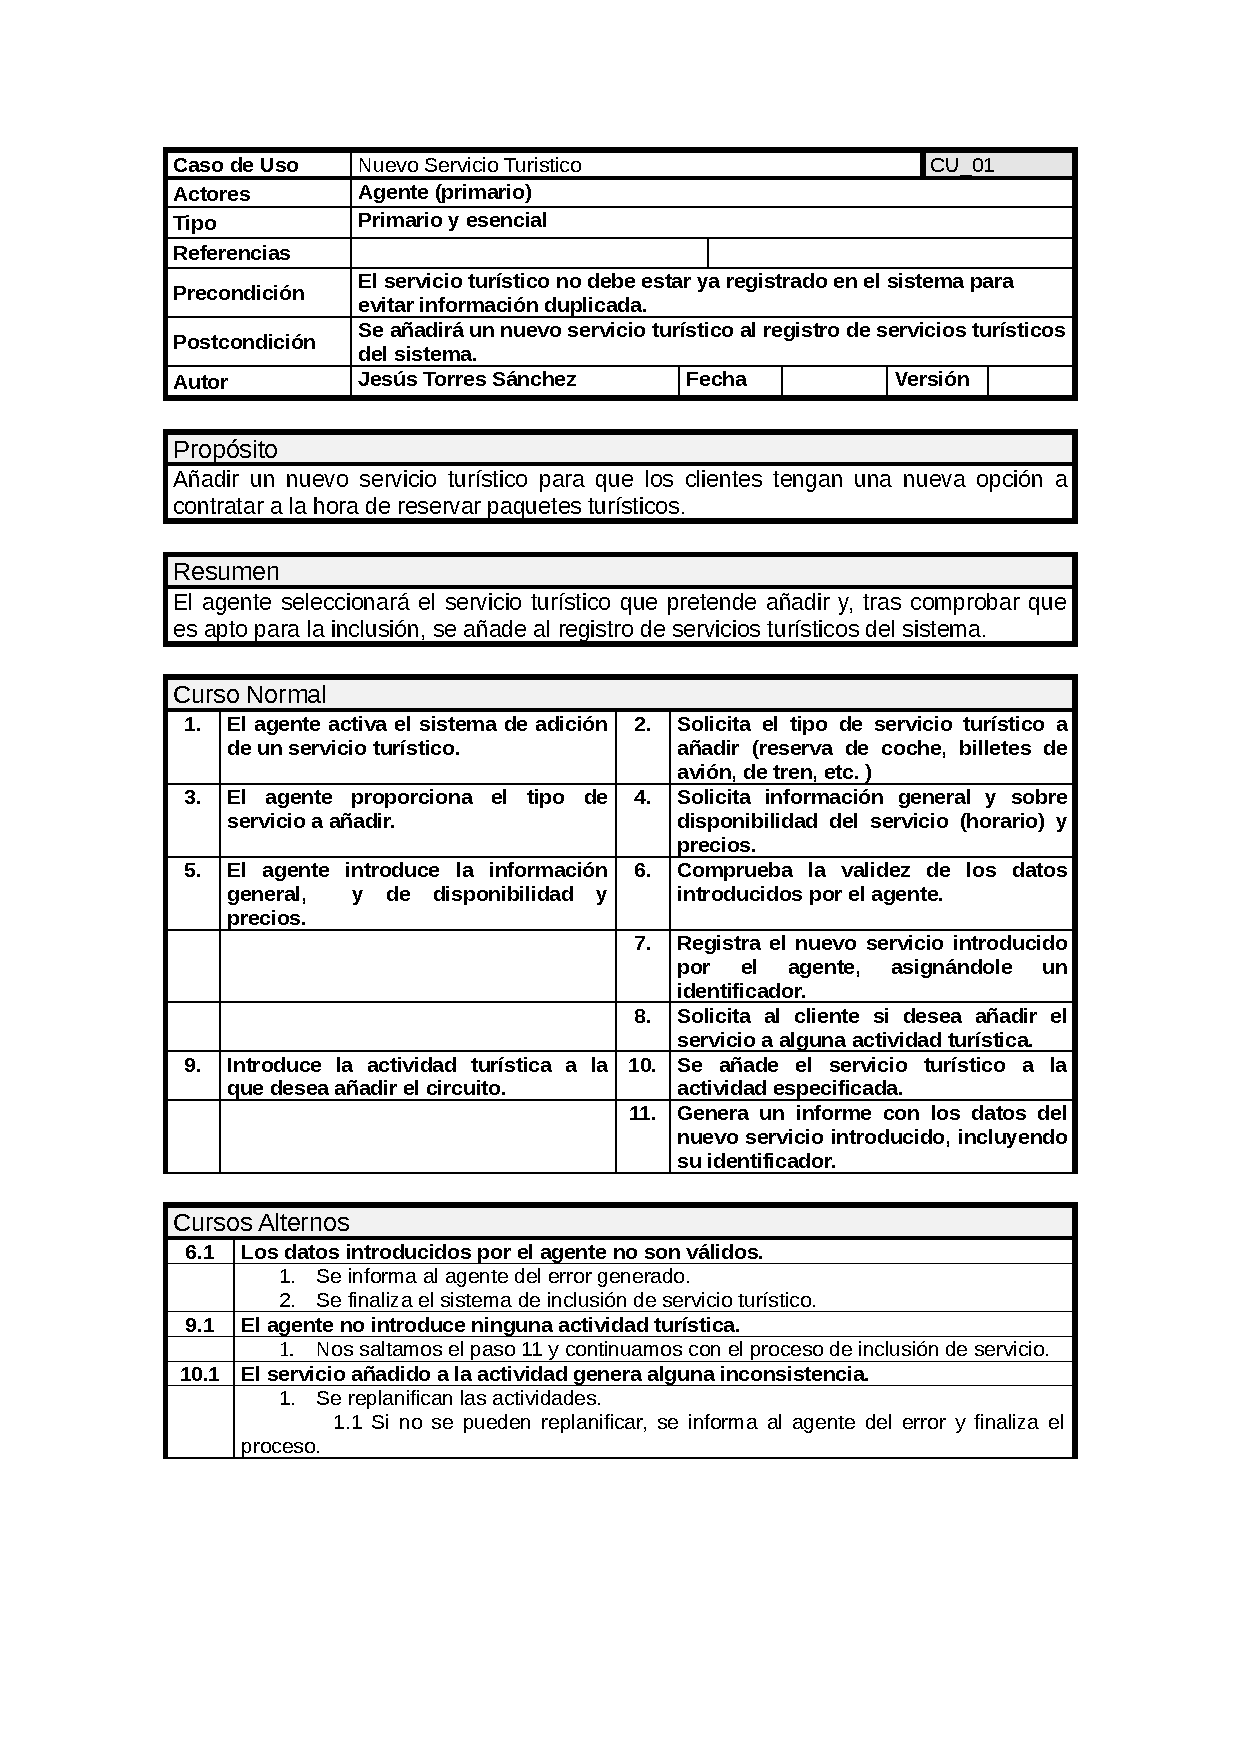
\includepdf[page={2-12}]{cu-jesus}
	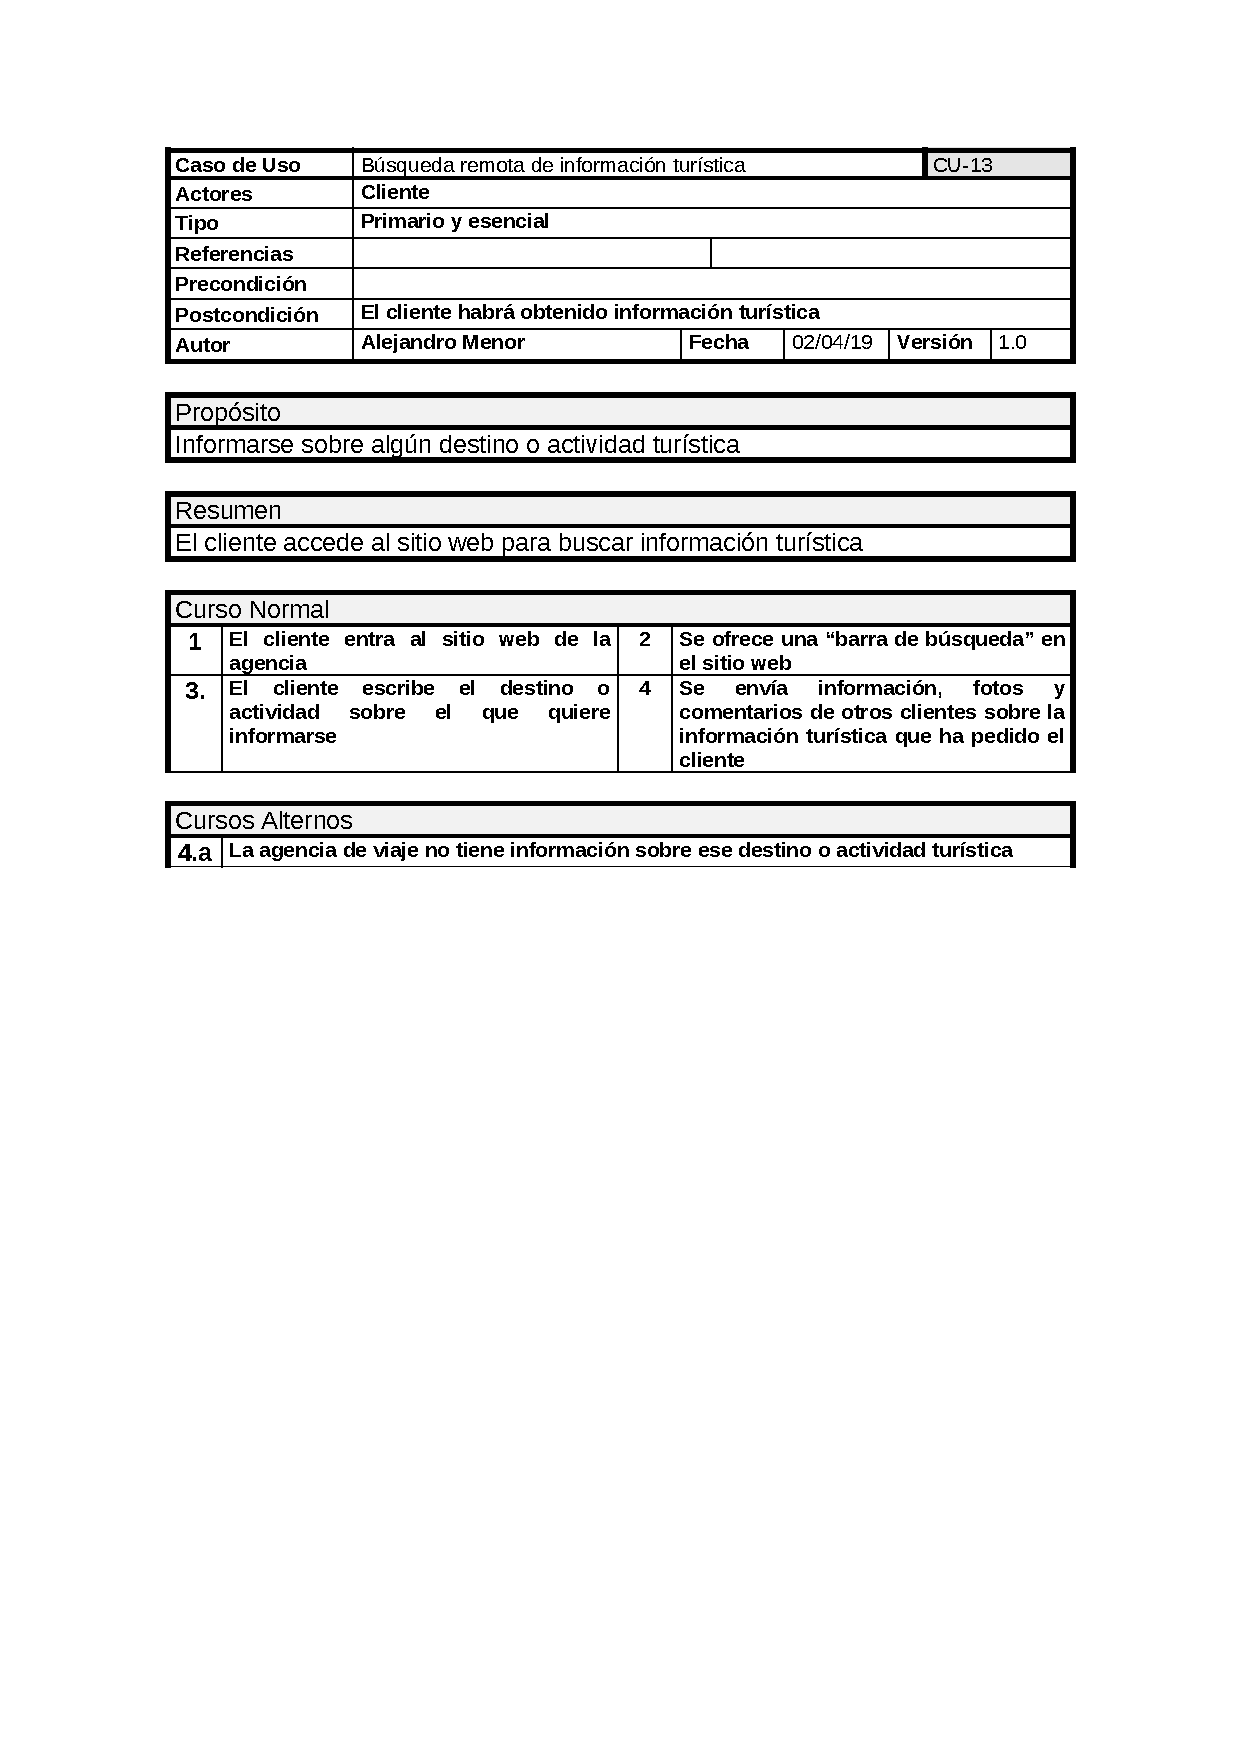
\includepdf[page={-}]{cu-alex}
	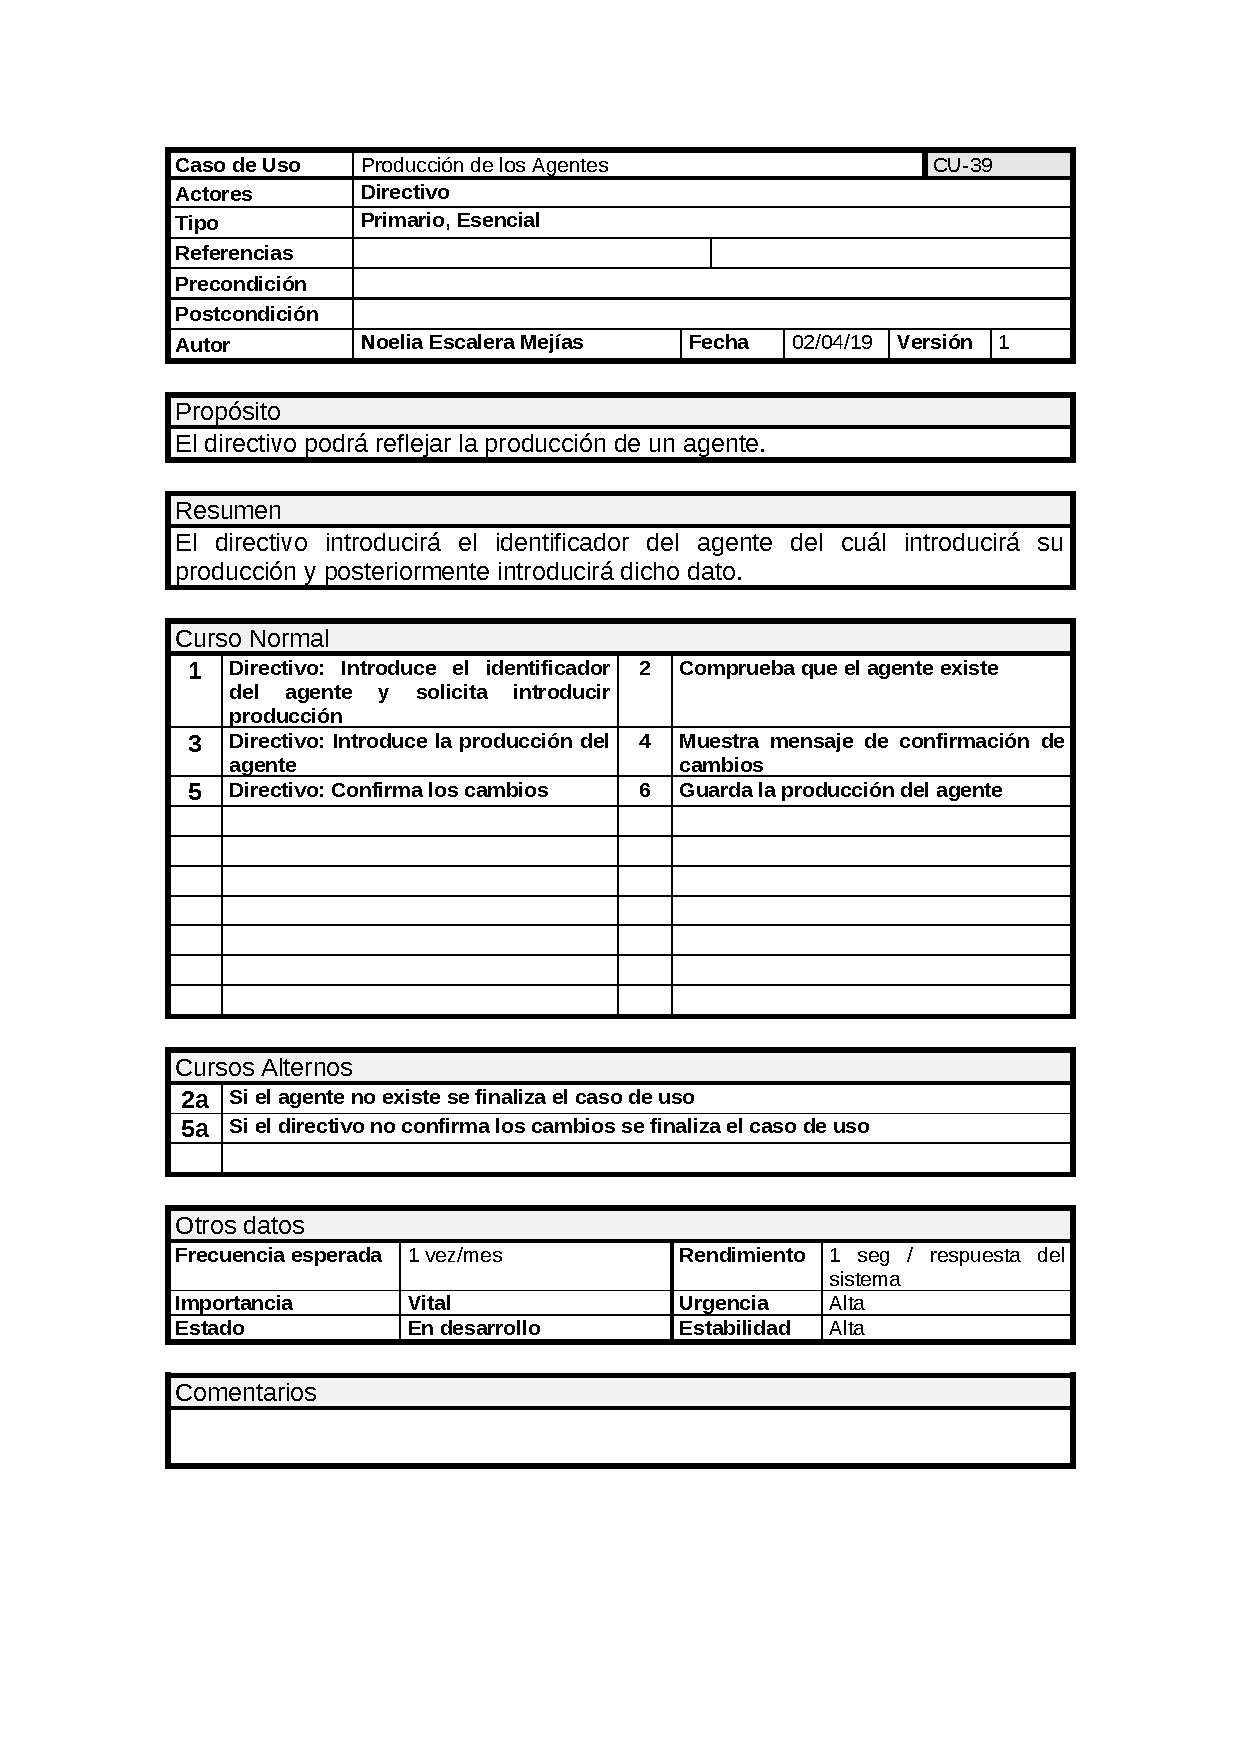
\includepdf[page={-}]{cu-noelia}
	
	\section{Diagrama de actividad}
	\begin{figure}[H]
		\centering
		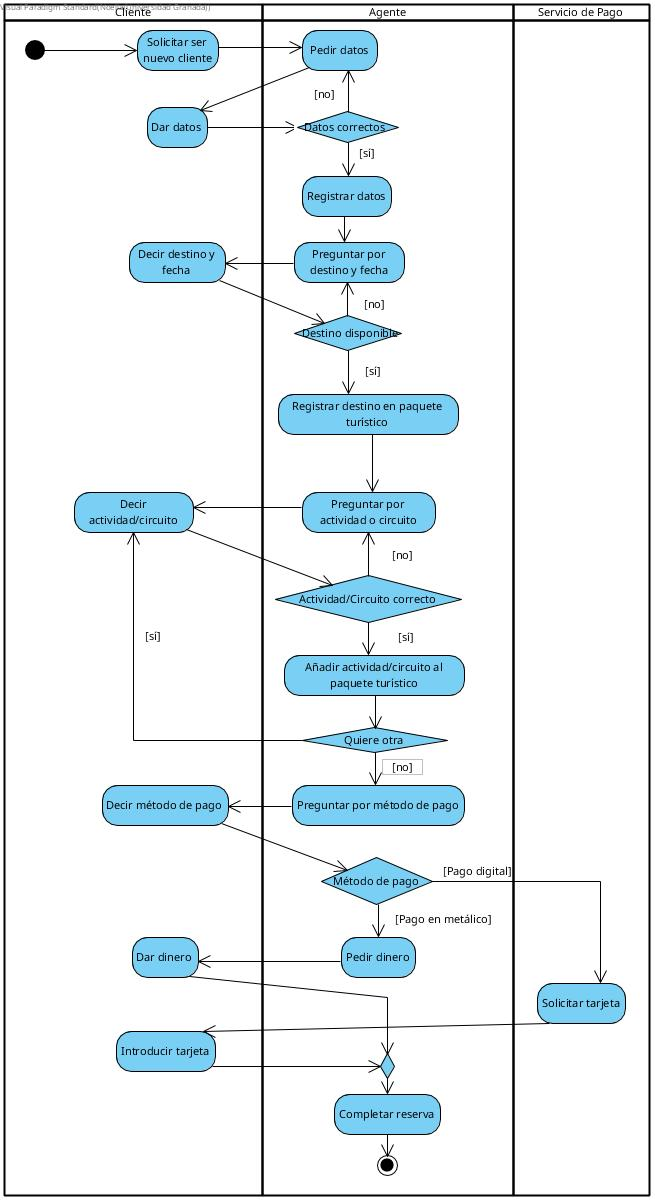
\includegraphics[totalheight=16cm]{Actividad}
	\end{figure}
	\section{Glosario de términos extendido}
	\begin{itemize}
		\item \textbf{Servicio turístico.} Cualquiera de los servicios que oferta la a agencia.
		\item \textbf{Actividad turística.} Conjunto de servicios turísticos.
		\item \textbf{Circuito turístico.} Conjunto de actividades turísticas.
		\item \textbf{Paquete turístico.} Conjunto de servicios, actividades y circuitos turísticos para un cliente o grupo de clientes.
		\item \textbf{Grupo.} Conjunto de clientes con un paquete turístico en común.
		\item \textbf{Observación.} Comentario a añadir sobre un agente determinado.
		\item \textbf{Abono.} Pago parcial.
		\item \textbf{Lista de distribución.} Publicidad y ofertas que se enviarán a un grupo de usuarios.
	\end{itemize}
\end{document}